\chapter{Misure con oscilloscopio digitale su amplificatore operazionale in configurazione catena chiusa}
\label{chap:terza_prova}

\section*{Obiettivo}
\label{sec:ob_third}
L'obiettivo della terza esperienza di laboratorio è quello di valutare la frequenza di taglio e il guadagno di un amplificatore operazionale in configurazione a \emph{catena chiusa} (closed-loop) al fine di effettuare il tracciamento della risposta in frequenza del circuito integrato in questione.

\section{L'amplificatore operazionale µA741}
L'amplificatore operazionale (OP-AMP) è un dispositivo attivo, dotato cioè di alimentazione, in grado  di amplificare i segnali in ingresso. Durante l'esperienza è stato usato l'OP-AMP µA471, provvisto dei seguenti pin:
\begin{itemize}
    \item V\textsubscript{+} morsetto non invertente
    \item V\textsubscript{-} morsetto invertente
    \item V\textsubscript{o} pin d'uscita
    \item +V\textsubscript{cc} e -V\textsubscript{cc} pin per l'alimentazione in continua
    \item due pin per la compensazione dell'offset
\end{itemize}

\begin{figure}
    \centering
    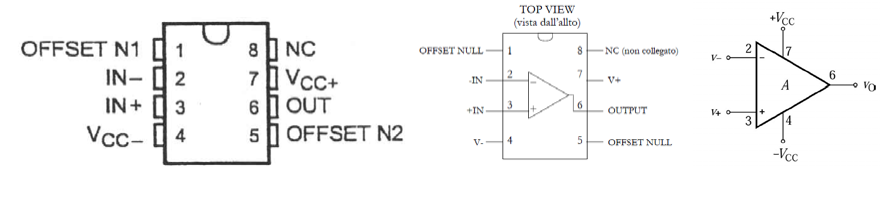
\includegraphics[width=1\linewidth]{media/uA741.png}
    \caption{Piedinatura e schema interno del $\mu$A741}
    \label{fig:Piedinatura e schema interno del uA741}
\end{figure}
\FloatBarrier
\section{Caratterizzazione µA741 in catena chiusa}
Dalle specifiche del µA741, si può osservare che questo circuito integrato richiede un’alimentazione duale compresa tra ±9V e ±15V.

\subsubsection{Gain Bandwidth Product (GBWP) – Prodotto banda-guadagno}
Il GBWP di un amplificatore operazionale è il prodotto tra il modulo del suo guadagno ad anello aperto e la frequenza di taglio a 3 dB. In pratica, è la frequenza a cui il guadagno di tensione ad anello aperto si riduce al valore unitario. Questo parametro (caratteristico per ciascun amplificatore), essendo costante a qualsiasi
frequenza, permette di determinare il massimo guadagno ottenibile da uno strumento ad una determinata frequenza, e viceversa. Dal grafico disponibile sul datasheet dell’amplificatore, Figura \ref{fig:Diagramma Avd vs Frequenza},  si osserva che ad un guadagno di 0 dB ad anello aperto corrisponde una frequenza pari ad 1 MHz.
Pertanto si può determinare la banda passante (B) e la frequenza di taglio teorica (f\textsubscript{c}):
\[f_c=B=\frac{GBWP}{|A|}\]
\begin{figure}[h]
    \centering
    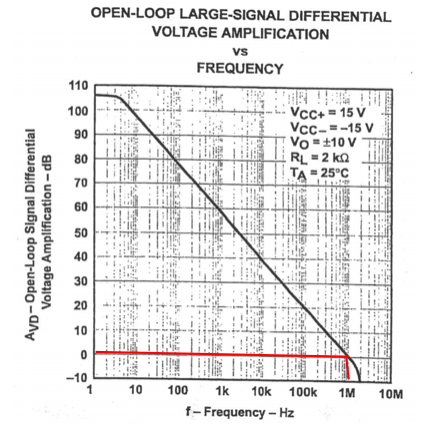
\includegraphics[width=0.5\linewidth, height=7cm]{diagrammaOLvsFreq_uA741.png}
    \caption{Diagramma $A_{VD}$ vs Frequenza}
    \label{fig:Diagramma Avd vs Frequenza}
\end{figure}
\FloatBarrier
\clearpage

\subsection{Tensione di offset e compensazione}
Idealmente, un amplificatore differenziale alimentato con una tensione duale e con ingressi collegati entrambi a massa, dovrebbe fornire in uscita una tensione pari a 0 V. In realtà, invece, esistono sempre delle dissimmetrie interne di funzionamento che danno origine ad una piccola tensione d’uscita, cioè la “tensione di offset”. Pertanto, data la non idealità dell'OP-AMP, i pin 1 e 5 devono essere regolati, facendo riferimento allo schema in Figura \ref{fig:Piedinatura e schema interno del uA741}. Sperimentalmente, l’effetto dell’offset può essere osservato effettuando i seguenti passaggi:

\begin{enumerate}
    \item Attraverso l'alimentatore da banco HP E3631A (Figura \ref{fig:HPE3631A}) , è stata impostata un'alimentazione di ±12V. Questa operazione, è stata effettuata premendo su Output ON, poi  su +25V e successivamente, effettuando la regolazione con la manopola presente sul generatore, viene impostato il valore +12V. Analogamente si procede nella stessa maniera per impostare il valore -12V, sfruttando il tasto -25V.  Si è poi premuto Output OFF per mantenere il valore di alimentazione in memoria. L'uscita COM dell'alimentatore da banco è stata collegata poi tramite un connettore BNC al circuito integrato. Infine si può premere nuovamente il tasto Output ON. 
    \item Spegnendo il generatore di funzione a cui è collegato il circuito integrato non si fornisce alcun segnale agli ingressi;
    \item  Sull’oscilloscopio, si visualizza solo il canale al quale è collegato l’uscita dell’amplificatore operazionale.
    \item  Il segnale visualizzato è in continua, con sovrapposto un segnale di rumore (Figura \ref{fig:tensioneOffset}): per questo, è opportuno eseguire una misura mediata della tensione efficace (\textit{Misura RMS}), andando a selezionare prima il tasto \textit{Measure} e successivamente il tasto \textit{RMS}.
    \item  Per compensare l’offset in modo da riportare a 0 V la tensione in uscita, è necessario collegare fra i due pin interessati (offset o balance), un trimmer il cui cursore risulti collegato alla tensione di alimentazione oppure a massa.
    \item Regolare tale trimmer fino a rilevare in uscita una tensione nulla (Figura \ref{fig:azzeramentoOffset}). 
\end{enumerate}

Operativamente, per annullare l’offset, si utilizza il trimmer già presente sul circuito fornito durante l’esercitazione: tramite un cacciavite, si ruota la vite presente fin quando non vengono letti valori dell’ordine di pochi µV.  Per tale operazione si imposta  sul canale d'uscita una  $K_v$ molto bassa in modo da visualizzare  poche decine di mV per divisione.
  
Nel caso dell'esperienza, è stato fissato un valore pari a:

\[V_{rms}=866,4 \mu V\]
\FloatBarrier
\begin{figure}
    \centering
    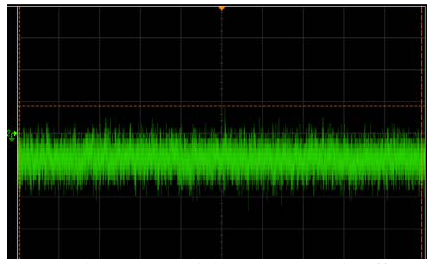
\includegraphics[width=0.5\linewidth]{media/tensioneOffest.png}
    \caption{Tensione di offest vista sull'scilloscopio}
    \label{fig:tensioneOffset}
\end{figure}
\begin{figure}
    \centering
    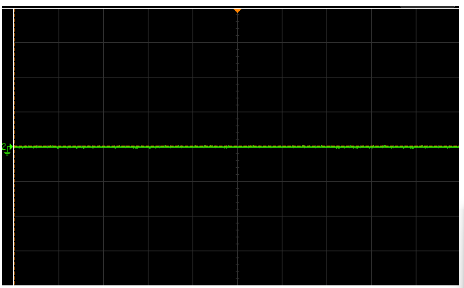
\includegraphics[width=0.5\linewidth]{media/azzeramentoOffset.png}
    \caption{Azzeramento dell'offset visto sull'oscilloscopio}
    \label{fig:azzeramentoOffset}
\end{figure}
\FloatBarrier

\subsection{Guadagno teorico e frequenza di taglio teorica in catena chiusa}

Il circuito nella configurazione “a catena chiusa” è stato realizzato direttamente su un PCB (Printed Circuit Board) ossia una scheda elettronica, di cui la schematizzazione è in Figura \ref{fig:schemaCatenaChiusa}:
\begin{figure}[h]
    \centering
    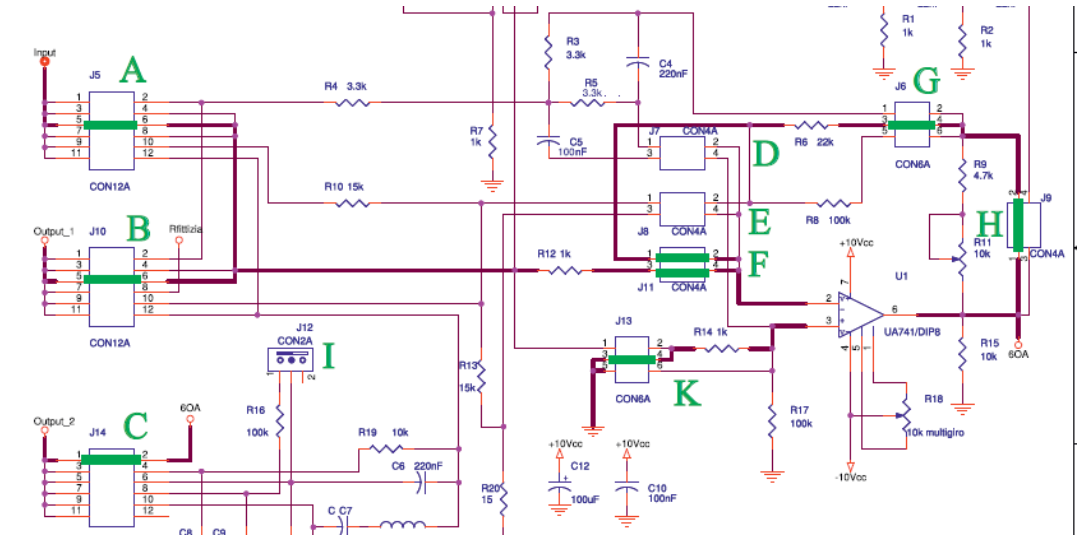
\includegraphics[width=1\linewidth]{media/schemaCircuitaleuA741.png}
    \caption{Schema circuitale della configurazione in catena chiusa}
    \label{fig:schemaCatenaChiusa}
\end{figure}
\FloatBarrier
Al fine di abilitare la configurazione catena chiusa dell'amplificatore operazionale sono stati utilizzati dei Jumper (tratti spessi in verde ) che sono stati posizionati come indicato in Figura.
\FloatBarrier
Nel circuito di interesse, la resistenza \(R_6\) (tra ingresso invertente dell’amplificatore ed il pin di uscita) ed \(R_{12}\) (tra ingresso invertente dell’amplificatore ed ingresso dell’amplificatore) determinano il guadagno teorico in catena chiusa dell’amplificatore, che vale:

\[A_{Teorico}=-\frac{R_6}{R_{12}}=-\frac{22 k\Omega}{1 k\Omega}=-22\]

La resistenza \(R_{14}\) posta tra l’ingresso non invertente e massa serve per non collegare direttamente l’ingresso non invertente a massa, ma ad un valore di resistenza prossimo a quello dell’ingresso invertente. La resistenza variabile \(R_{18}\) (da 10 k\(\Omega\)) è di tipo multi-giro e serve a compensare il valore di tensione di offset. Dopo aver ridotto l’offset, e stimato il segnale di ingresso in ampiezza e frequenza, per mezzo del generatore di funzioni si fornisce in ingresso al circuito un segnale sinusoidale. Partendo da questo valore di ampiezza, si varia l’ampiezza del segnale (aumentandola o diminuendola) fino ad ottenere la massima tensione d’uscita picco-picco. Se l’ampiezza del segnale supera il valore massimo, l’amplificatore raggiunge la regione di saturazione.
Invece, la frequenza di taglio teorica \(f_{c_{teorica}}\), si ricava dalla relazione già espressa precedentemente, per cui:

\[f_{c_{teorica}}=\frac{GBWP}{|A|}=45,5kHz\]
\subsection{Strumentazione}
Di seguito è riportata la strumentazione utilizzata per la realizzazione del set-up di questa esperienza di laboratorio.

\subsection*{\textbf{PCB}}

\subsection*{\textbf{Oscilloscopio Agilent HP 54600B}}
\begin{figure}[h]
    \centering
    \includegraphics[width=0.8\linewidth, height=7cm]{oscilloscopio.png}
    \caption{Oscilloscopio Agilent HP 54600B}
    \label{fig:enter-label}
\end{figure}
\FloatBarrier
\subsection*{\textbf{Generatore di funzioni HP 33120A}}
\begin{figure}[h]
    \centering
    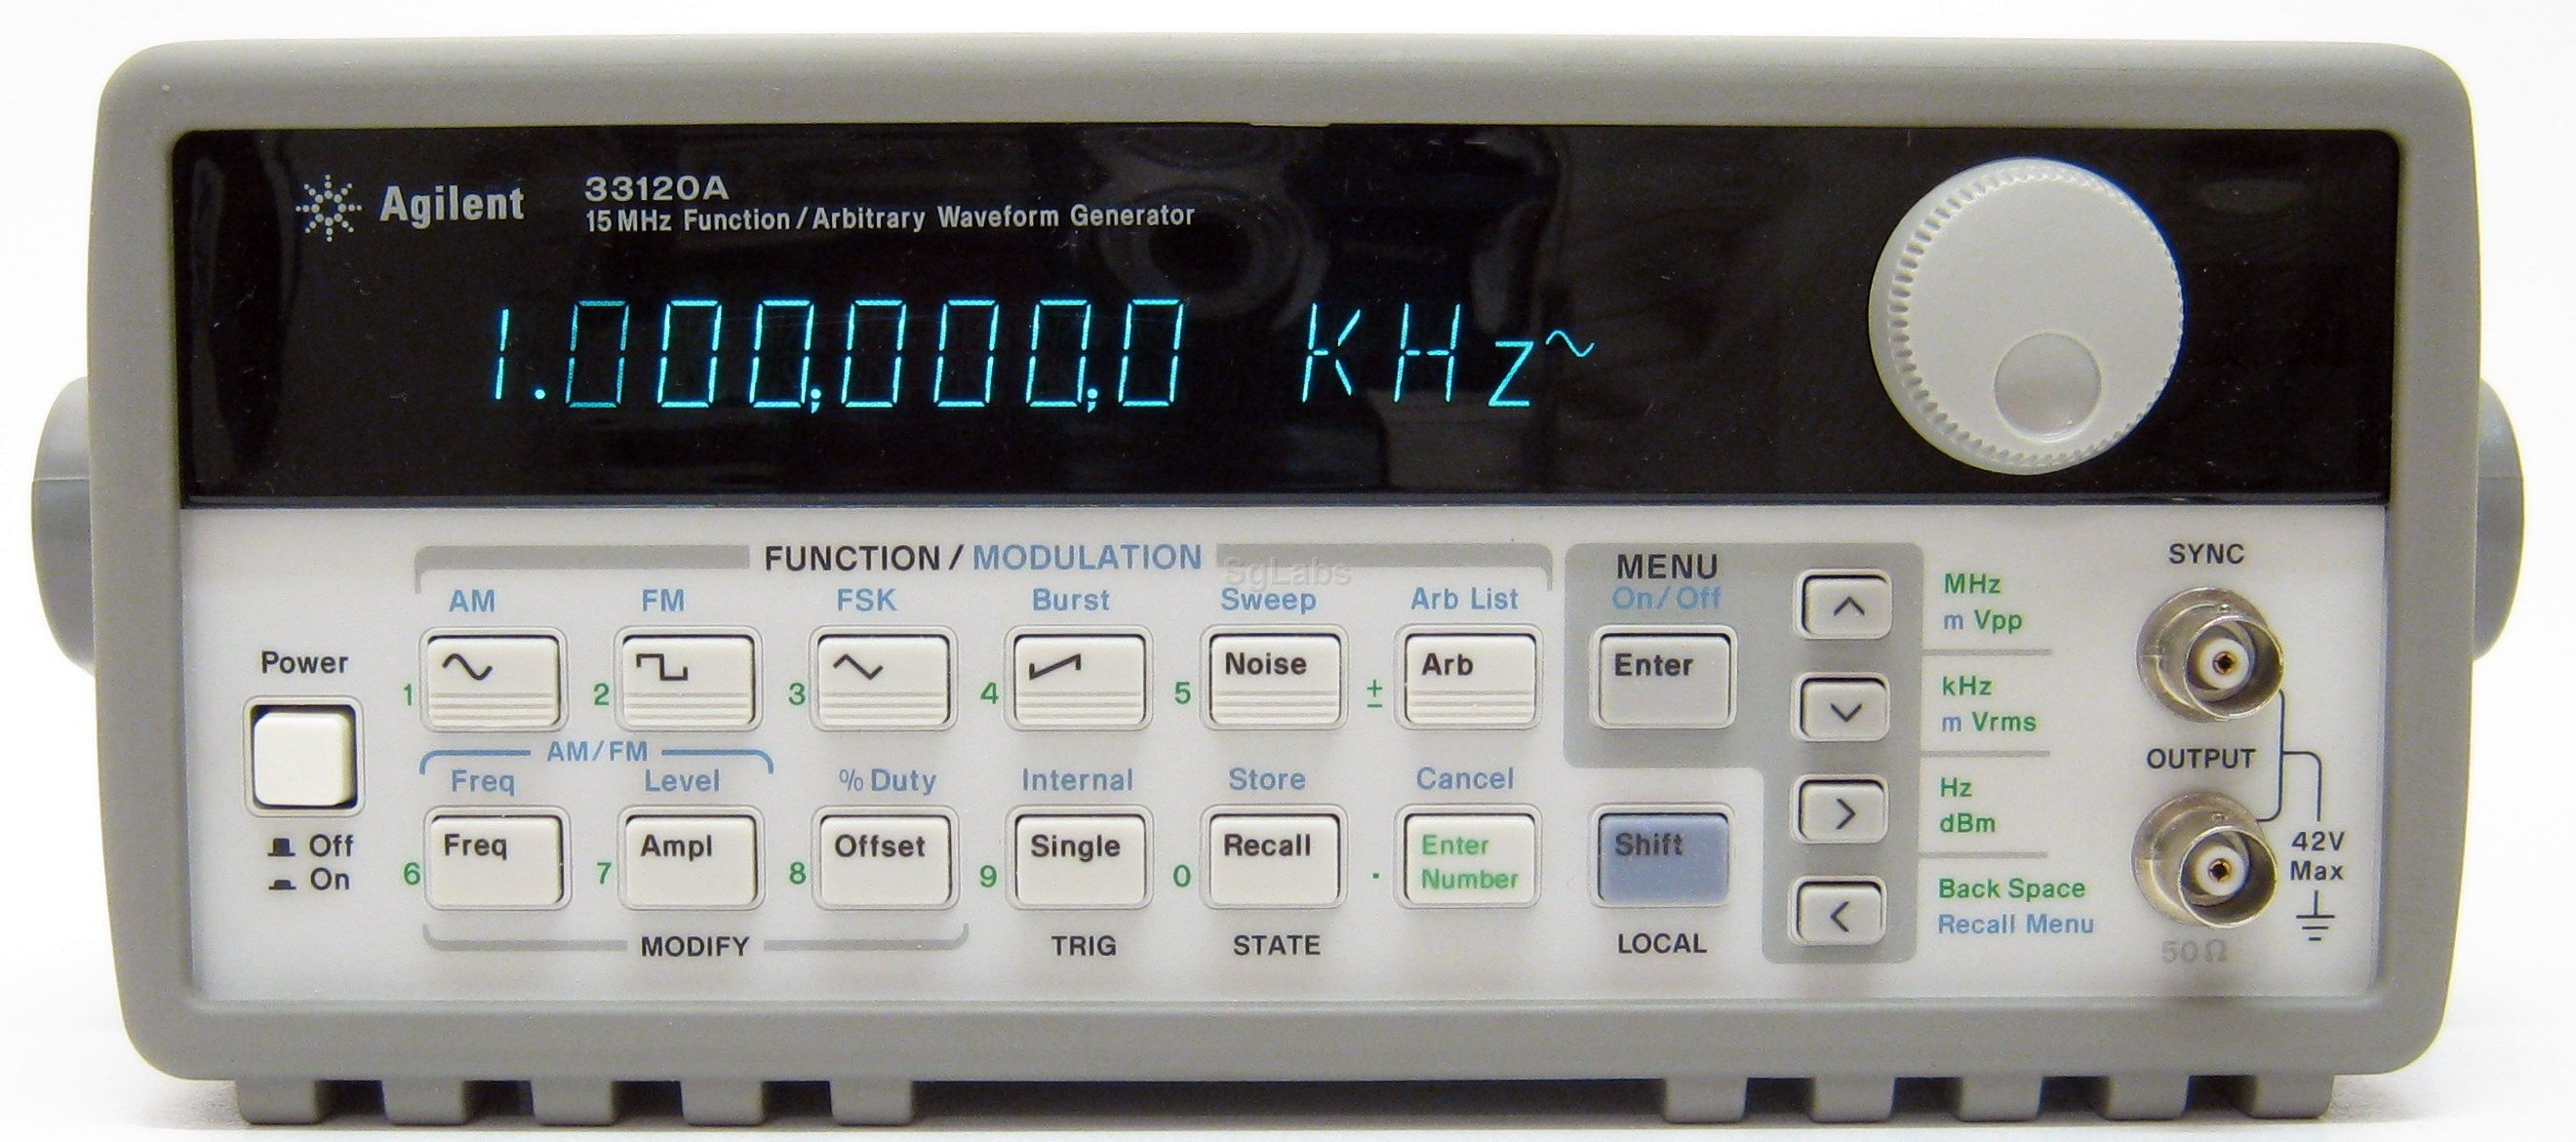
\includegraphics[width=0.9\linewidth, height=6cm]{generatore di funzioni.png}
    \caption{Generatore di funzioni HP 33120A}
    \label{fig:enter-label}
\end{figure}
\FloatBarrier
\subsection*{\textbf{Alimentatore da banco HP E3631A}}
\begin{figure}[h]
    \centering
    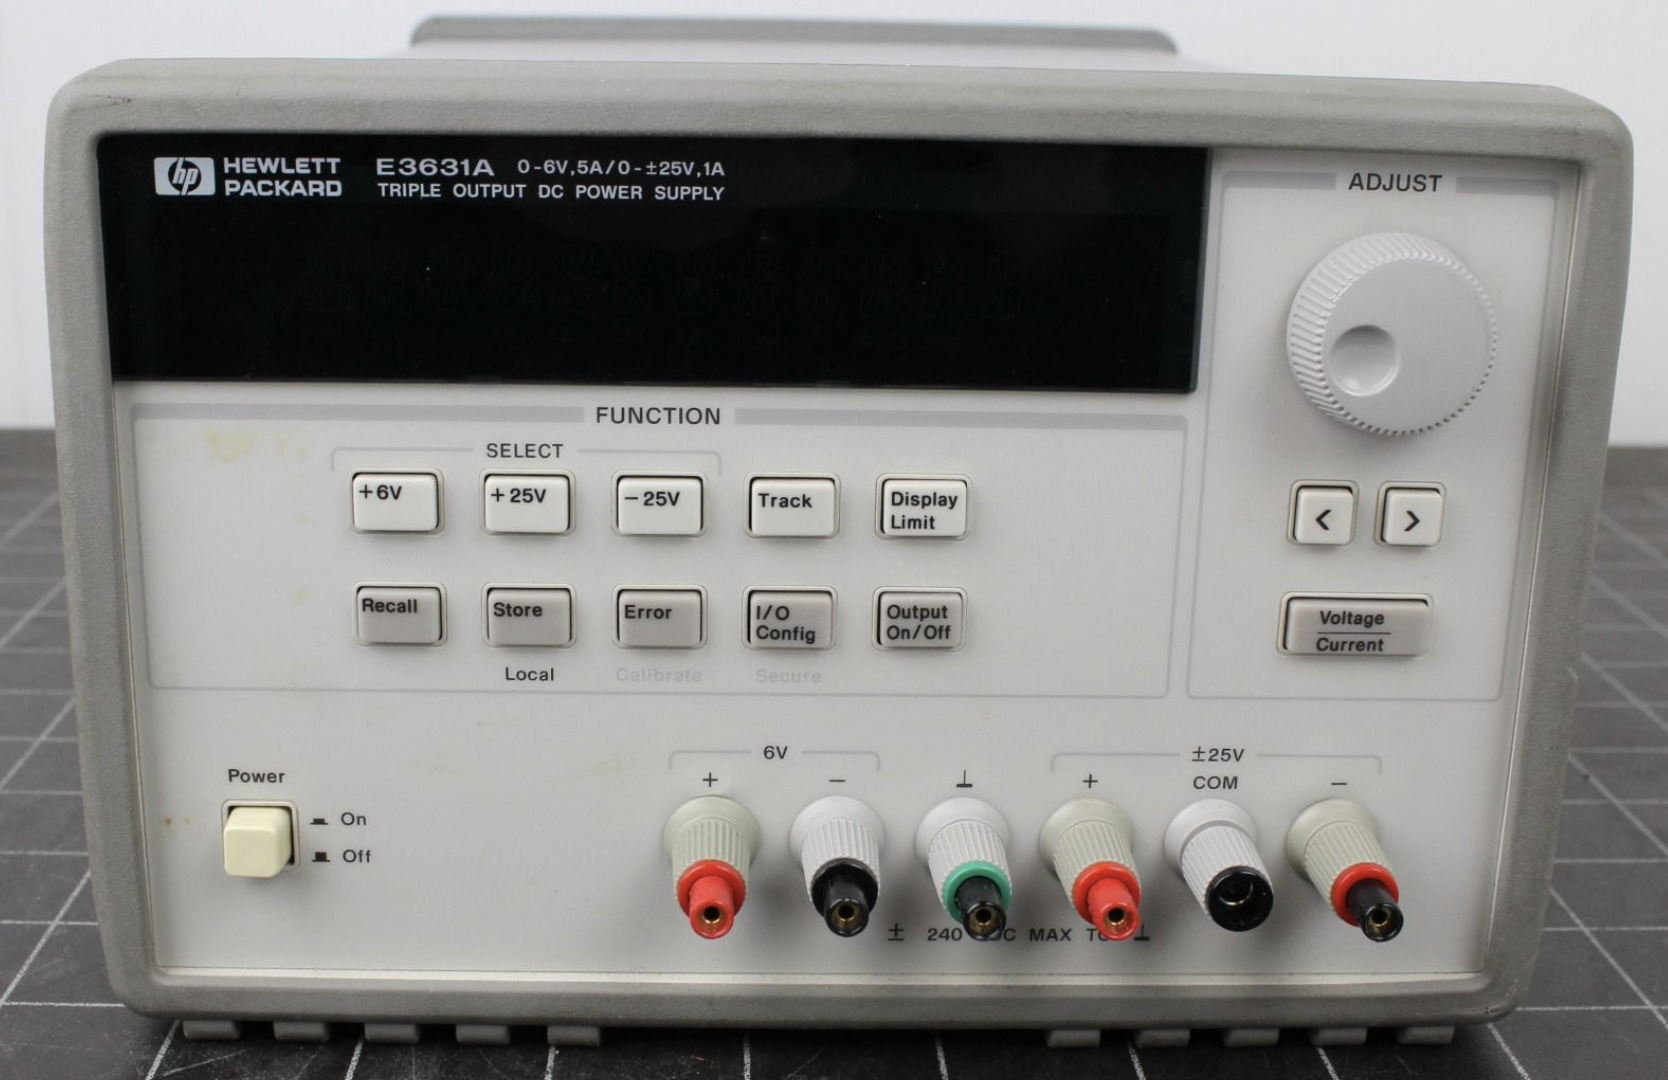
\includegraphics[width=0.8\linewidth, height=7cm]{alimentatore da banco.png}
    \caption{Alimentatore da banco HP E3631A}
    \label{fig:HPE3631A}
\end{figure}
\FloatBarrier
\subsection*{\textbf{Cavi di connessione BNC-BNC}}
\begin{figure}[h]
    \centering
    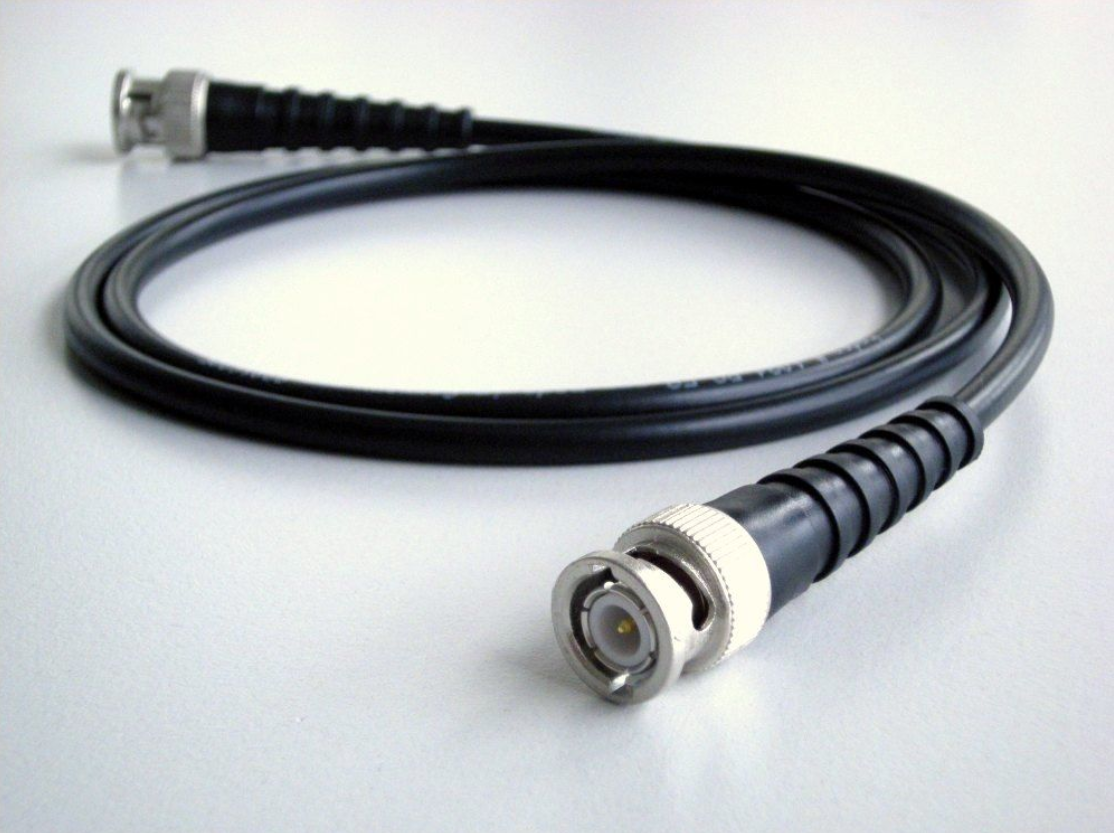
\includegraphics[width=0.75\linewidth]{media/cavoBNC.png}
    \caption{Cavo di connessione BNC-BNC}
    \label{fig:enter-label}
\end{figure}
\FloatBarrier
\clearpage

\subsection{Configurazione della strumentazione per le misurazioni}
Prima di iniziare ad effettuare le misurazioni del caso, abbiamo configurato tutte le strumentazioni a disposizione. Abbiamo dunque:
\begin{itemize}
    \item Collegato i cavi di connessione BNC-BNC secondo la seguente configurazione:
    \begin{itemize}
        \item Uscita del generatore di funzioni Agilent HP 54600B all'ingresso (INPUT) del circuito integrato
        \item  Segnale di ingresso all'operazionale (OUTPUT 1) è stato collegato al canale 1 dell'oscilloscopio
        \item  Segnale di uscita dall'operazionale (OUTPUT 2) è stato collegato al canale 2 dell'oscilloscopio
        \item Uscita COM dell'alimentatore da banco HP E3631A all'ingresso, del circuito integrato, che si trova in altro a destra, facendo riferimento a Figura \ref{fig:pcb_bnc}
    \end{itemize}
    \item Al fine di controllare il corretto funzionamento dell'amplificatore abbiamo si è impostato sul generatore un segnale di ingresso sinusoidale alla frequenza di $100Hz$ e si è visto come il segnale d'uscita fosse sfasato ed amplificato di all'incirca $20dB$.  
\end{itemize}
\begin{figure}[h]
        \centering
        \includegraphics{PCB_bnc.png}
        \caption{Ingressi/Uscite del filtro RC}
        \label{fig:pcb_bnc}
    \end{figure}
\FloatBarrier
E' importante osservare che l'ampiezza visualizzata sull'oscilloscopio è diversa da quella impostata sul generatore di funzioni a causa del disadattamento di impedenza tra l'oscilloscopio ed il generatore di funzioni.
\begin{itemize}
    \item Avviato l'oscilloscopio su cui visualizzare il segnale d'ingresso dell'operazionale $V_i$ sul canale 1, e il segnale di uscita dell'operazionale $V_o$ sul canale 2.
    Poichè abbiamo utilizzato cavi BNC-BNC e non sonde, abbiamo impostato il valore di \emph{Probe} a 1 mediante l'apposito pulsante posto sotto lo schermo.
    Per migliorare la visualizzazione di entrambi i segnali, abbiamo premuto il pulsante \emph{Auto-Scale}, che permette all'oscilloscopio di visualizzare entrambi i segnali, uno per ognuno della due metà dello schermo.
    
    Ai fini delle misurazioni da effettuare, abbiamo impostato entrambe le forme d'onda sulla linea di 0 V secondo la seguente procedura per entrambi i canali:
    \begin{enumerate}
        \item Selezione del singolo canale dal rispettivo pulsante della sezione verticale
        \item Impostazione del \emph{Coupling} su \textit{Ground} mediante il secondo pulsante posizionato sotto lo schermo
        \item Utilizzo della manopola presente sotto la sezione \textit{Measure} per spostare il riferimento del segnale sulla linea di 0 V
        \item Impostazione del \emph{Coupling} su \textit{AC} mediante il secondo pulsante posizionato sotto lo schermo  
\end{enumerate}
\end{itemize}


\subsection{Misurazioni}
\subsubsection{Calcolo della frequenza di taglio sperimentale}
Per la valutazione sperimentale del guadagno, serve effettuare la stima delle tensioni picco-picco \(V_{o,pp}\)
e \(V_{i, pp}\) attraverso l'utilizzo dell'oscilloscopio. Da queste due stime si è ottenuto:

\[V_{o,pp}=4,125V\]

\[V_{i, pp}=190,6mV\]
Da cui:

\[A=-\frac{V_{o,pp}}{V_{i, pp}}=-21,6\]
Andando a determinare quanto vale A, in corrispondenza della frequenza di taglio \(f_c\), tale per cui si ha un'attenuazione di 3dB, segue che:

\[A_{-3dB}=\frac{A}{\sqrt{2}}=-15,27\]
Infine, è possibile calcolare il valore della tensione di uscita in corrispondenza della frequenza di
taglio, facendo uso della relazione:

\[V_o=A_{-3dB} \cdot V_i=2,91V_{pp}\]
Per la valutazione sperimentale della frequenza di taglio, si impostano i due cursori orizzontali dell’oscilloscopio in corrispondenza di questo valore di tensione. Si procede quindi a variare la frequenza del segnale fino a che il segnale in uscita visualizzato sull’oscilloscopio non risulta tangente ai due cursori orizzontali. In corrispondenza della frequenza di taglio, si può notare che il segnale in uscita è distorto (segnale triangolare) e che il valore di frequenza trovato è diverso dal valore teorico. Questo succede perché si sta lavorando con un segnale di ingresso con ampiezza massima. Per evitare questo effetto, è necessario ridurre l’ampiezza del segnale, ricalcolare il nuovo valore di attenuazione a 3dB e, quindi, stimare la frequenza di taglio. In questo caso, si è trovato che \(f_c=33kHz\).
\clearpage
\subsubsection{Misure di tensione picco-picco}

Per riuscire a ricavare la risposta in frequenza del circuito, è stato necessario ripetere la stessa procedura di misura, lasciando invariate le condizioni operative, per un totale di 24 diversi valori di frequenza.

Per ogni misurazione abbiamo quindi eseguito i seguenti passi:
\begin{enumerate}
    \item Impostato il valore della frequenza del segnale di ingresso del filtro  sul generatore di funzioni, premendo prima il pulsante \emph{Freq} e poi impostando la frequenza desiderata.
    \item Regolato i valori di $K_{V_i}$ e $K_{V_o}$ mediante le manopole poste nella parte superiore della sezione verticale, in modo tale che i segnali si avvicinassero quanto più possibile al valore di fondo scala. In questo modo le misure eseguite sono più accurate e viene ridotta l'incertezza di misura.
    \item Premuto il pulsante \emph{Voltage}, situato nella sezione \emph{Measure} e selezionato per ognuno dei due segnali il tipo di misura, cioè tensione picco-picco $V_{pp}$, mediante gli appositi pulsanti posizionati sotto lo schermo.
    In questo modo i valori di tensione picco-picco di entrambi i segnali $V_i$ e $V_o$ vengono automaticamente calcolati dall'oscilloscopio e visualizzati nella parte inferiore dello schermo.

Di seguito una tabella con i risultati delle misurazioni effettuate:
    
\end{enumerate}
\begin{table}[!ht]
    \centering
    \begin{tabular}{|c|c|c|c|c|c|}
    \hline

        \textbf{FREQ [Hz]} & $\bm{V_i(mV)}$ & $\bm{KV_i(mV)}$ & $\bm{V_o(mV)}$ & $\bm{KV_o(mV)}$ & \textbf{A} \\ \hline

      
        100 & 190,6 & 50 & 4156,0 & 1000 & 21,805  \\ \hline
        1000 & 190,6 & 50 & 4125,0 & 1000 & 21,642  \\ \hline
        10000 & 192,2 & 50 & 3969,0 & 1000 & 20,650 \\ \hline
        15000 & 190,2 & 50 & 3797,0 & 500 & 19,755  \\ \hline
        20000 & 193,8 & 50 & 3578,0 & 500 & 18,462 \\ \hline
        25000 & 193,8 & 50 & 3328,0 & 500 & 17,172  \\ \hline
        30000 & 193,8 & 50 & 3094,0 & 500 & 15,965  \\ \hline
        35000 & 195,3 & 50 & 2884,0 & 500 & 14,767  \\ \hline
        40000 & 196,9 & 50 & 2625,0 & 500 & 13,332  \\ \hline
        45000 & 196,9 & 50 & 2422,0 & 500 & 12,301  \\ \hline
        50000 & 196,9 & 50 & 2250,0 & 500 & 11,427  \\ \hline
        100000 & 200 & 50 & 1231,0 & 200 & 6,155  \\ \hline
        150000 & 200 & 50 & 843,8 & 200 & 4,219  \\ \hline
        200000 & 200 & 50 & 643,8 & 100 & 3,219  \\ \hline
        250000 & 200 & 50 & 512,5 & 100 & 2,563  \\ \hline
        300000 & 200 & 50 & 431,2 & 100 & 2,156  \\ \hline
        350000 & 200 & 50 & 367,2 & 50 & 1,836	\\ \hline																				
        400000	& 200 & 50 & 321,9 & 50 & 1,610	\\ \hline																			
        450000	& 200	& 50	& 284,4	& 50	& 1,422 \\ \hline													
        500000 &	200 &	50 &	256,2 &	50 &	1,281	\\ \hline							
        550000 &	200 &	50 &	232,8 &	50 &	1,164 \\ \hline																		
        600000 &	200 &	50 &	212,5 &	50 &	1,063	\\ \hline																
        650000 &	200 &	50 &	196,9 &	50 &	0,985 \\ \hline																
        700000 &	200 &	50 &	181,2 &	50 &	0,906	\\ \hline																
        
    \end{tabular}
\end{table}


% scrivere le formuke usate per ricavare incertezze ib ase ai datasheet
% piccolo excursus su cosa sono quei valori
% mettere tabelle di excel


\subsection{Calcolo delle incertezze}
In questo paragrafo si effettuerà sulle misure ottenute la valutazione dell'incertezza di \textbf{tipo B}, basata sull'utilizzo di informazioni note a priori quali le specifiche metrologiche degli strumenti adoperati.

\subsubsection{Misure Dirette}

Le misure dirette effettuate durante l'esperienza di laboratorio sono le seguenti:
\begin{itemize}
    \item \textbf{tensione picco-picco V}
    \item \textbf{frequenza f} dei segnali $V_i$ e $V_o$ 
\end{itemize}


\subsubsection*{Incertezza associata alle misure di tensione picco-picco V}

Dalle specifiche metrologiche di ampiezza dell'oscilloscopio, poichè abbiamo utilizzato i due cursori orizzontali per le misure, consideriamo la \textbf{Dual cursor accuracy}, pari a 
\[vertical \ accuracy \pm 0.4\% \ of full scale\]

dove \textbf{vertical accuracy} per l'oscilloscopio Agilent HP 54600B è pari a 1.9\%, mentre \textbf{full scale} è il fondo scala del dispositivo ed è pari a $y_{FS} = 8 \cdot k_v$, dove 8 sono le divisioni verticali e $k_v$ è la \emph{vertical sensitivity} espressa in V/div.

La \emph{Dual cursor accuracy} sopra riportata deriva dalla formula generale dell'incertezza per una differenza 
\[U(V_1 - V_2) = U_G|V_1 - V_2| + 2U_{inl} + 2U{q}\]

Nel nostro caso, l'incertezza di non linearità integrale $U_{inl}$, è stata conglobata nel termine 1.9\% insieme a $U_G$ incertezza di guadagno. L'incertezza di quantizzazione $2U_q$ è invece pari al termine $\pm 0.4\% \cdot y_{FS}$. L'incertezza di offset $U_O$ non è presente poichè nel caso di differenze di misure l'errore di offset si compensa.

Indicato quindi con $V$ il valore di tensione picco-picco letto, l'\textbf{incertezza di caso peggiore} associata a $V$ è data dalla seguente formula:

\[U_V = \frac{1.9}{100} \cdot |V| + \frac{0.4}{100} \cdot 8 \cdot k_v\]

Da questa formula è possibile poi ricavare l'\textbf{incertezza relativa di caso peggiore}:
\[U_{r,V} = \frac{U_V}{V}\]

Seguono due tabelle contenenti per ogni valore di frequenza: il valore di tensione letto, la vertical sensitivity all'atto della lettura, l'incertezza assoluta di caso peggiore e l'incertezza relativa di caso peggiore.

%due tabelle per Vi e Vo 

\begin{table}[!ht]
    \centering
    \begin{tabular}{|c|c|c|c|c|}
    \hline

        \textbf{FREQ [Hz]} & $\bm{V_i(mV)}$ & $\bm{KV_i(mV)}$ & $\bm{U(V_i)}$ & $\bm{U_r(V_i)}$  \\ \hline

      
100	& 190,6	& 50 &	0,005221 &	0,00002739 \\ \hline
1000	& 190,6 &	50 &	0,005221 &	0,00002739 \\ \hline
10000	& 192,2	& 50 &	0,005252 &	0,00002732 \\ \hline
15000	& 192,2	& 50 &	0,005252 &	0,00002732 \\ \hline
20000	& 193,8 &	50 &	0,005282 &	0,00002726 \\ \hline
25000	& 193,8 &	50 &	0,005282 &	0,00002726 \\ \hline
30000	& 193,8 &	50 &	0,005282 &	0,00002726 \\ \hline
35000	& 195,3 &	50 &	0,005311 &	0,00002719 \\ \hline
40000	& 196,9 &	50 &	0,005341 &	0,00002713 \\ \hline
45000	& 196,9 &	50 &	0,005341 &	0,00002713 \\ \hline
50000	& 196,9	& 50 &	0,005341 &	0,00002713 \\ \hline
100000	& 200	& 50 &	0,005400 &	0,00002700 \\ \hline
150000	& 200	& 50 &	0,005400 &	0,00002700 \\ \hline
200000	& 200	& 50 &	0,005400 &	0,00002700 \\ \hline
250000	& 200	& 50 &	0,005400 &	0,00002700 \\ \hline
300000	& 200	& 50 &	0,005400 &	0,00002700 \\ \hline
350000	& 200	& 50 &	0,005400 &	0,00002700 \\ \hline
400000	& 200	& 50 &	0,005400 &	0,00002700 \\ \hline
450000	& 200	& 50 &	0,005400 &	0,00002700 \\ \hline
500000	& 200	& 50 &	0,005400 &	0,00002700 \\ \hline
550000	& 200	& 50 &	0,005400 &	0,00002700 \\ \hline
600000	& 200	& 50 &	0,005400 &	0,00002700 \\ \hline
650000	& 200	& 50 &	0,005400 &	0,00002700 \\ \hline
700000	& 200	& 50 &	0,005400 &	0,00002700	\\ \hline												
        
    \end{tabular}
\end{table}

\begin{table}[!ht]
    \centering
    \begin{tabular}{|c|c|c|c|c|}
    \hline

        \textbf{FREQ [Hz]} & $\bm{V_o(mV)}$ & $\bm{KV_o(mV)}$ & $\bm{U(V_o)}$ & $\bm{U_r(V_o)}$  \\ \hline

      
100	& 4156,0 &	1000	& 0,1110 &	0,00002670  \\ \hline
1000 & 4125,0 & 1000	& 0,1104 &	0,00002676  \\ \hline
10000 & 3969,0 & 1000	& 0,1074 &	0,00002706  \\ \hline
15000	& 3797,0 &	500	& 0,0881 &	0,00002321  \\ \hline
20000	& 3578,0 &	500	& 0,0840 &	0,00002347  \\ \hline
25000	& 3328,0 &	500	& 0,0792 &	0,00002381  \\ \hline
30000	& 3094,0 &	500	& 0,0748 &	0,00002417  \\ \hline
35000	& 2884,0 &	500	& 0,0708 &	0,00002455  \\ \hline
40000	& 2625,0 &	500	& 0,0659 &	0,00002510  \\ \hline
45000	& 2422,0 &	500	& 0,0620 &	0,00002561  \\ \hline
50000	& 2250,0 &	500	& 0,0588 &	0,00002611  \\ \hline
100000	& 1231,0 &	200	& 0,0298 &	0,00002420  \\ \hline
150000	& 843,8	 &  200	& 0,0224 &	0,00002658  \\ \hline
200000	& 643,8	 & 100	& 0,0154 &	0,00002397  \\ \hline
250000	& 512,5	 & 100 &	0,0129 &	0,00002524  \\ \hline
300000	& 431,2 &	100 &	0,0114 &	0,00002642  \\ \hline
350000	& 367,2	& 50 &	0,0086	& 0,00002336  \\ \hline
400000	& 321,9	& 50 &	0,0077	& 0,00002397  \\ \hline
450000	& 284,4	& 50 &	0,0070	& 0,00002463  \\ \hline
500000	& 256,2	& 50 &	0,0065	& 0,00002525  \\ \hline
550000	& 232,8	& 50 &	0,0060	& 0,00002587   \\ \hline
600000	& 212,5	& 50 &	0,0056	& 0,00002653  \\ \hline
650000	& 196,9	& 50 &	0,0053	& 0,00002713  \\ \hline
700000	& 181,2	& 50 &	0,0050	& 0,00002783		 \\ \hline									
        
    \end{tabular}
\end{table}

\clearpage
\subsubsection{Misure Indirette}

L'unica misura indiretta eseguita è il \textbf{guadagno A}.

\subsubsection*{Incertezza associata alle misure del guadagno $A$}

Ricordiamo che il guadagno $A$ dell'amplificatore operazionale è definito come
\[A = \frac{V_o}{V_i}\]
cioè è data dal rapporto di due misure dirette. Pertanto, per poter stimare l'incertezza di $A$, occorre ricorrere alla \textit{formula di propagazione delle incertezze di caso peggiore}:
\[U = \sum_{n=1}^{N} \left|\frac{\partial f}{\partial y_i}\right| \cdot U_i\]

Dall'applicazione di tale formula, nel caso di rapporto tra misure, si ha che l'\textbf{incertezza relativa} è data dalla \textbf{somma delle incertezze relative} delle singole misure dirette. Pertanto nel nostro caso essa è pari a:

\[U_{r,A} = U_{r,V_o} + U_{r,V_i}\]

da cui si ha\textbf{ l'incertezza assoluta di caso peggiore}:

\[U_A = A \cdot U_{r,A}\]

Solitamente i valori di guadagno $A$ vengono riportati in dB(decibel) secondo la formula:

\[A_{dB} = 20\cdot \log_{10} A\]

Applicando la formula di propagazione dellle incertezze si ottiene l'espressione per l'\textbf{incertezza assoluta di caso peggiore} $U_{A_{db}}$:

\[U_{A_{db}} = \frac{20}{\ln 10} \cdot U_{r,A}\]

Segue la tabella riportante per ogni valore di frequenza: il valore calcolato di $A$ con relativa incertezza (assoluta e relativa) di caso peggiore e il valore in dB di $A$ con relativa incertezza assoluta di caso peggiore


\begin{table}[!ht]
    \centering
    \begin{tabular}{|c|c|c|c|c|c|c|}
    \hline
        \textbf{f (Hz)} & \textbf{A} & \textbf{U(A)} & $\bm{U_r(A)}$ & $\bm{A_{dB}}$ & $\bm{U(A_{dB})}$ & $\bm{U_r(A_{dB})}$ \\ \hline
        100 & 21,805 & 0,001180 & 0,0000541 & 26,771 & 0,000470 & 0,0000176 \\ \hline
        1000 & 21,642 & 0,001172 & 0,0000542 & 26,706 & 0,000470 & 0,0000176 \\ \hline
        10000 & 20,650 & 0,001123 & 0,0000544 & 26,299 & 0,000472 & 0,0000180 \\ \hline
        15000 & 19,755 & 0,000998 & 0,0000505 & 25,914 & 0,000439 & 0,0000169 \\ \hline
        20000 & 18,462 & 0,000937 & 0,0000507 & 25,326 & 0,000441 & 0,0000174 \\ \hline
        25000 & 17,172 & 0,000877 & 0,0000511 & 24,697 & 0,000444 & 0,0000180 \\ \hline
        30000 & 15,965 & 0,000821 & 0,0000514 & 24,063 & 0,000447 & 0,0000186 \\ \hline
        35000 & 14,767 & 0,000764 & 0,0000517 & 23,386 & 0,000449 & 0,0000192 \\ \hline
        40000 & 13,332 & 0,000696 & 0,0000522 & 22,498 & 0,000454 & 0,0000202 \\ \hline
        45000 & 12,301 & 0,000649 & 0,0000527 & 21,799 & 0,000458 & 0,0000210 \\ \hline
        50000 & 11,427 & 0,000608 & 0,0000532 & 21,159 & 0,000462 & 0,0000219 \\ \hline
        100000 & 6,155 & 0,000315 & 0,0000512 & 15,785 & 0,000445 & 0,0000282 \\ \hline
        150000 & 4,219 & 0,000226 & 0,0000536 & 12,504 & 0,000465 & 0,0000372 \\ \hline
        200000 & 3,219 & 0,000164 & 0,0000510 & 10,154 & 0,000443 & 0,0000436 \\ \hline
        250000 & 2,563 & 0,000134 & 0,0000522 & 8,173 & 0,000454 & 0,0000555 \\ \hline
        300000 & 2,156 & 0,000115 & 0,0000534 & 6,673 & 0,000464 & 0,0000695 \\ \hline
        350000 & 1,836 & 0,000092 & 0,0000504 & 5,277 & 0,000437 & 0,0000829 \\ \hline
        400000 & 1,610 & 0,000082 & 0,0000510 & 4,134 & 0,000443 & 0,0001071 \\ \hline
        450000 & 1,422 & 0,000073 & 0,0000516 & 3,058 & 0,000448 & 0,0001466 \\ \hline
        500000 & 1,281 & 0,000067 & 0,0000522 & 2,151 & 0,000454 & 0,0002110 \\ \hline
        550000 & 1,164 & 0,000062 & 0,0000529 & 1,319 & 0,000459 & 0,0003482 \\ \hline
        600000 & 1,063 & 0,000057 & 0,0000535 & 0,527 & 0,000465 & 0,0008830 \\ \hline
        650000 & 0,985 & 0,000053 & 0,0000541 & -0,136 & 0,000470 & -0,0034649 \\ \hline
        700000 & 0,906 & 0,000050 & 0,0000548 & -0,857 & 0,000476 & -0,0005554 \\ \hline
    \end{tabular}
\end{table}